\documentclass{beamer}
\usetheme{metropolis}
\usepackage{graphicx}
\usepackage{subfig}
\title{Algebra-Based Physics-1: Mechanics (PHYS135A-01): Unit 1}
\date{\today}
\author{Jordan Hanson}
\institute{Whittier College Department of Physics and Astronomy}

\begin{document}
\maketitle

\section{Unit 0 Review}

\begin{frame}{Unit 0 Review}
\begin{enumerate}
\item Methods of approximation
\begin{itemize}
\item \alert{Estimating} the correct order of magnitude
\item \alert{Function} approximation
\item \alert{Unit analysis}
\end{itemize}
\item Coordinates and vectors
\begin{itemize}
\item \alert{Scalars} and \alert{vectors}
\item \alert{Cartesian} (rectangular) coordinates, displacement
\item \alert{Vector} addition, subtraction, and multiplication
\end{itemize}
\item Review of geometry and trigonometry techniques
\begin{itemize}
\item Similar triangles
\item Pythagorean theorem
\item Sine, cosine, tangent ...
\end{itemize}
\end{enumerate}
\end{frame}

\section{Unit 1 Summary}

\begin{frame}{Unit 1 Summary}
\begin{enumerate}
\item Displacement, average velocity and acceleration
\begin{itemize}
\item \textit{Mathematics review}: slope of a function
\end{itemize}
\item The case of constant acceleration
\begin{itemize}
\item An \textit{an equation of motion} for constant acceleration
\item Derivation of \alert{common equations of motion}
\item Average quantities and exercises
\end{itemize}
\item \textbf{Lab Activity: Measuring acceleration of gravity: \textit{g}}
\item Exercises with vectors, graphs, and equations of motion
\end{enumerate}
\end{frame}

\section{Displacement, average velocity and acceleration}

\begin{frame}{Displacement, average velocity and acceleration}
\begin{figure}
\centering
\subfloat[\label{fig:twovectors_a}]{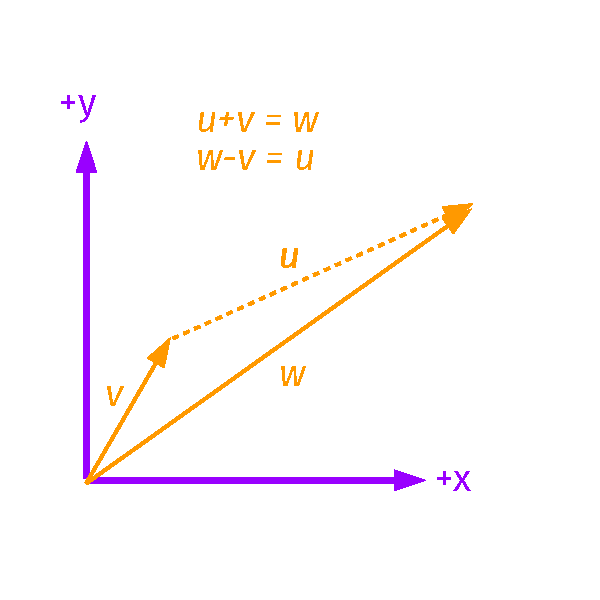
\includegraphics[width=0.45\textwidth]{figures/Vectors4.pdf}}
\subfloat[\label{fig:twovectors_b}]{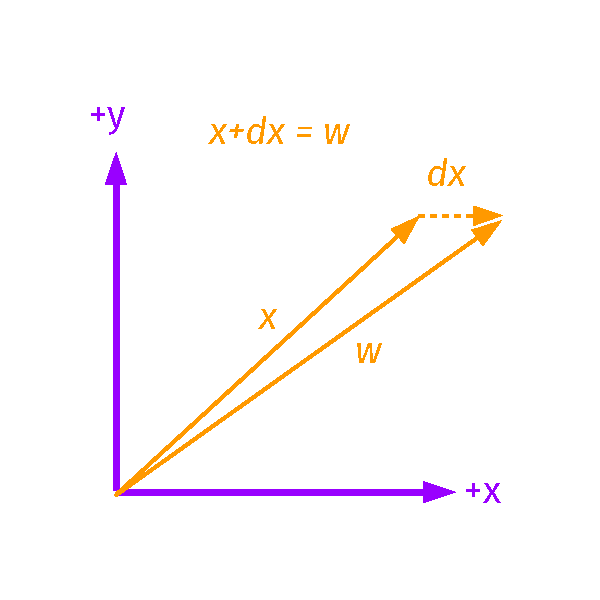
\includegraphics[width=0.45\textwidth]{figures/Vectors1.pdf}}
\caption{\label{fig:displacement} (Left): The displacement vector is $\vec{u}$.  (Right) Treat displacement for a small change in time, $dt$, and call it $d\vec{x}$.}
\end{figure}
\end{frame}

\begin{frame}{Mathematics Review: slope of a function}
\begin{figure}
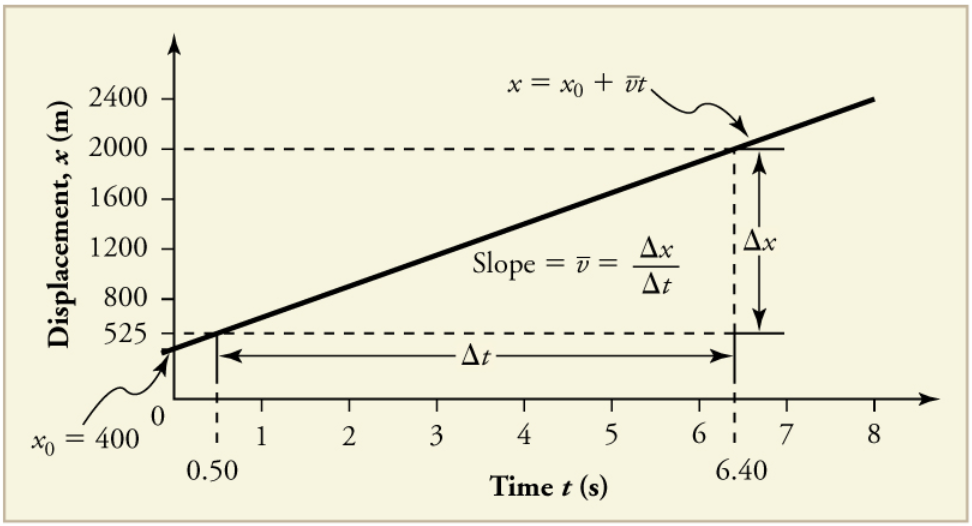
\includegraphics[width=0.8\textwidth]{figures/slope.png}
\caption{\label{fig:slope} We can think of the velocity of a system as the \textit{slope} of the displacement versus time.}
\end{figure}
\end{frame}

\begin{frame}{Displacement, and average velocity and acceleration}
Definition of average velocity vector:
\begin{equation}
\boxed{\bar{v} = \frac{\Delta\vec{x}}{\Delta t}}
\end{equation} \\
\vspace{0.5cm}
Simple example: Let the initial and final positions of a particle be 4.0 m and 8.0 m, and the initial and final times be 0.0 sec and 8.0 sec.  Then we have 
\begin{align}
\Delta \vec{x} &= 8.0 - 4.0 = 4.0 \quad m \\
\Delta t &= 8.0 - 0.0 = 8.0 \quad sec
\end{align}
Then
\begin{equation}
\bar{v} = 4.0/8.0 = 0.5 \quad m/s
\end{equation}
\end{frame}

\begin{frame}{Displacement, and average velocity and acceleration}
Definition of average \textit{acceleration} vector:
\begin{equation}
\boxed{\bar{a} = \frac{\Delta \vec{v}}{\Delta t}}
\end{equation} \\
\vspace{0.5cm}
Simple example: Let the initial and final velocity of a system be 2.0 m/s and 3.0 m/s, and the initial and final times be 0.0 sec and 1.0 sec.  Then we have
\begin{align}
\Delta \vec{v} &= 3.0 - 2.0 = 1.0 \quad m/s \\
\Delta t &= 1.0 - 0.0 = 1.0 \quad sec
\end{align}
Then
\begin{equation}
\bar{a} = 1.0/1.0 = 1.0 \quad m/s^2
\end{equation}
\end{frame}

\begin{frame}{Displacement, and average velocity and acceleration}
\begin{columns}[T]
\begin{column}{0.5\textwidth}
\small
These quantities are examples of rates, derived from initial and final states. \\
\vspace{1cm}
The situation at right depicts an object that initially travels upward, but under the acceleration of gravity. \\
\vspace{1 cm}
Notice that \textit{constant} acceleration yields linear velocity and quadratic displacement (a property of calculus).
\end{column}
\begin{column}{0.5\textwidth}
\begin{figure}
\centering
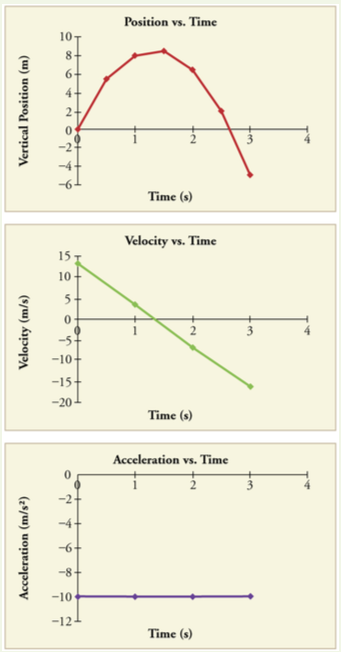
\includegraphics[width=0.6\textwidth]{figures/slope2.png}
\caption{\label{fig:slope2} Rate comparisons.}
\end{figure}
\end{column}
\end{columns}
\textbf{Professor: work several acceleration examples.}
\end{frame}

\begin{frame}{Displacement, and average velocity and acceleration}
A commuter backs her car out of her garage with an acceleration of 1.50 m/s$^2$.  How long does it take her to
reach a speed of 2.00 m/s?
\begin{itemize}
\item A: 1.0 s
\item B: 1.5 s
\item C: 1.33 s
\item D: 2.5 s
\end{itemize}
\end{frame}

\begin{frame}{Displacement, and average velocity and acceleration}
If she then brakes to a stop in 0.500 s, what is her deceleration?
\begin{itemize}
\item A: 4 m/s$^2$
\item B: -4 m/s$^2$
\item C: 2 m/s$^2$
\item D: -2 m/s$^2$
\end{itemize}
\end{frame}

\section{The case of constant acceleration}

\begin{frame}{The case of constant acceleration}
Consider the following three equations for a system experiencing constant acceleration:
\begin{align}
\vec{y}(t) &= (-\frac{1}{2}gt^2+v_{\rm i}t+y_{\rm 0}) \hat{j} \quad (m) \label{eq:threemain1} \\
\vec{v}(t) &= (-gt + v_{\rm i}) \hat{j} \quad (m/s) \label{eq:threemain2} \\
\vec{a}(t) &= (-g) \hat{j} \quad (m/s^2) \label{eq:threemain3}
\end{align}
What if we solve for time in Eq. \ref{eq:threemain2}, after taking the magnitude of the vector? \\
\begin{equation}
\frac{v-v_{\rm i}}{-g} = t
\label{eq:subt1}
\end{equation}
\end{frame}

\begin{frame}{The case of constant acceleration}
Now substitute Eq. \ref{eq:subt1} into Eq. \ref{eq:threemain1}:\\
\begin{align}
y &= -\frac{1}{2}g\left(\frac{v-v_{\rm i}}{-g}\right)^2+v_{\rm i}\left(\frac{v-v_{\rm i}}{-g}\right)+y_{\rm 0} \label{eq:threemain4} \\ 
-2g(y-y_{\rm 0}) &= (v-v_{\rm i})^2 + 2v_{\rm i}(v-v_{\rm i}) \label{eq:threemain5} \\
-2g(y-y_{\rm 0}) &= v^2-v_{\rm i}^2 \label{eq:threemain6} \\
-2g(y-y_{\rm 0})+v_{\rm i}^2 &= v^2 \label{eq:threemain7}
\end{align}
Equation \ref{eq:threemain7} provides a way to obtain the velocity of an accelerating system at some displacement without knowing the time.
\end{frame}

\begin{frame}{The case of constant acceleration}
A particle moves along the x-axis according to $x(t) = (10t-2t^2)\hat{i}$ m.  Where is the particle at 3.0 seconds?  What is the average velocity over the time inverval 0.0-3.0 seconds?
\begin{itemize}
\item A: 12 m, 4 m/s
\item B: 4 m, 12 m/s
\item C: 30 m, 4 m/s
\item D: 12 m, 12 m/s
\end{itemize}
\end{frame}

\begin{frame}{The case of constant acceleration}
Let $x(t) = (10t-2t^2)\hat{i}$ m, from prior exercise.  What is the displacement between $t=2$ seconds and $t=3$ seconds?  What is the average velocity in that period?
\begin{itemize}
\item A: 0 m, 0 m/s
\item B: 10 m, 10 m/s
\item C: 0 m, 4 m/s
\item D: 4 m, 0 m/s
\end{itemize}
\end{frame}

\begin{frame}{The case of constant acceleration}
Notice in the previous two problems: the \textit{instantaneous velocity} is not the \textit{average velocity}.  The average velocity between two and three seconds was 0 m/s, but the instantaneous velocity was not zero at either point.  However, the \textit{displacement} was 0 m in this time interval.  Take care not to confuse \textit{instantaneous} quantities with \textit{average} quantities.
\end{frame}

\begin{frame}{The case of constant acceleration}
\small
On February 15, 2013, a meteor entered Earth’s atmosphere over Chelyabinsk, Russia, and exploded at an altitude of 23.5 km.  Eyewitnesses could feel the intense heat from the fireball, and the blast wave from the explosion blew out windows in buildings. The blast wave took approximately 2 minutes 30 seconds to reach ground level.  What was the average velocity of the blast wave?  Compare this with the speed of sound, which is 343 m/s at sea level.
\begin{itemize}
\item A: 35 m/s (10\% speed of sound)
\item B: 100 m/s (30\% speed of sound)
\item C: 150 m/s (40\% speed of sound)
\item D: 350 m/s (100\% speed of sound)
\end{itemize}
\end{frame}

\begin{frame}{The case of constant acceleration}
\begin{align}
\vec{x}(t) &= \frac{1}{2}at^2+v_{\rm i}t+y_{\rm 0} \hat{j} \quad (m) \label{eq:summary1} \\
\vec{v}(t) &= at + v_{\rm i} \hat{j} \quad (m/s) \label{eq:summary2} \\
\vec{a} &= a \hat{j} \quad (m/s^2) \label{eq:summary3} \\
v_{\rm f}^2 - v_{\rm i}^2 &= 2a(x_{\rm f}-x_{\rm i}) \label{eq:summary4}
\end{align}
\end{frame}

\begin{frame}{The case of constant acceleration}
A particle moves along the x-axis according to $v(t) = (10-4t)\hat{i}$ m.  What is the average acceleration
between $t=2$ seconds and $t=3$ seconds?
\begin{itemize}
\item A: 4 m/s$^2$
\item B: 2 m/s$^2$
\item C: -2 m/s$^2$
\item D: -4 m/s$^2$
\end{itemize}
\end{frame}

\begin{frame}{The case of constant acceleration}
Same example.  What is the average acceleration between $t=0$ seconds and $t=3$ seconds?
\begin{itemize}
\item A: 4 m/s$^2$
\item B: 2 m/s$^2$
\item C: -2 m/s$^2$
\item D: -4 m/s$^2$
\end{itemize}
\end{frame}

\begin{frame}{The case of constant acceleration}
Notice that the \textit{average acceleration} doesn't depend on time (because it is constant).  Similar to the definition of \textit{average velocity}, we have the \textit{average acceleration}:\\
\begin{equation}
\bar{a} = \boxed{\frac{v_{\rm f} - v_{\rm i}}{t_{\rm f} - t_{\rm i}}}
\end{equation}
So if $a = constant$, $a(t) = \bar{a}$ and the numbers will always arrange themselves to give the same answer...
\end{frame}

\begin{frame}{The case of constant acceleration}
A cheetah can accelerate from rest to a speed of 35.0 m/s in 7.00 s. What is its average acceleration, if it's headed in the $-\hat{i}$ direction?
\begin{itemize}
\item A: -5 m/s$^2$
\item B: 2 m/s$^2$
\item C: 10 m/s$^2$
\item D: 5 m/s$^2$
\end{itemize}
\end{frame}

\begin{frame}{The case of constant acceleration}
Dr. John Paul Stapp was U.S. Air Force officer who studied the effects of extreme deceleration on the human body.  On December 10, 1954, Stapp rode a rocket sled, accelerating from rest to a top speed of 282 m/s (1015 km/h) in 5.00 s, and was brought jarringly back to rest in only 1.40 s!  Calculate his acceleration and deceleration. Express each in multiples of $g$, (9.8 m/s$^2$).
\begin{itemize}
\item A: 5.75 g's, 20.6 g's
\item B: 56.4 g's, 201 g's
\item C: 4.75 g's, 2.6 g's
\item D: 5.7 g's, 12.2 g's
\end{itemize}
\end{frame}

\begin{frame}{The case of constant acceleration}
While entering a freeway, a car accelerates from rest at a rate of 2.40 m/s$^2$ for 12.0 s.  How far does the car travel in that time?  What is the car’s final velocity?
\begin{itemize}
\item A: 14.4 m, 29 m/s
\item B: 346 m, 29 m/s
\item C: 173 m, 14.5 m/s
\item D: 173 m, 29 m/s
\end{itemize}
\end{frame}

\section{Lab Activity: Measuring acceleration of gravity}

\begin{frame}{Lab Activity: Measuring acceleration of gravity}
\small
\begin{figure}
\centering
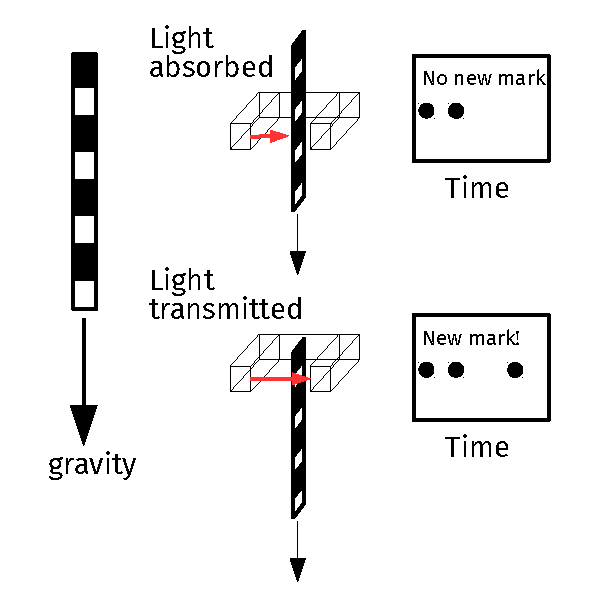
\includegraphics[width=0.5\textwidth]{figures/PicketG.pdf}
\caption{\label{fig:picket} (Left) A \textit{picket} is marked at regular intervals with black strips.  (Right) Upon dropping the picket through a \textit{photo-gate}, the strips will block the photo-gate and we will record when this happens on a clock.}
\end{figure}
\end{frame}

\begin{frame}{Lab Activity: Measuring acceleration of gravity}
\small
\begin{figure}
\centering
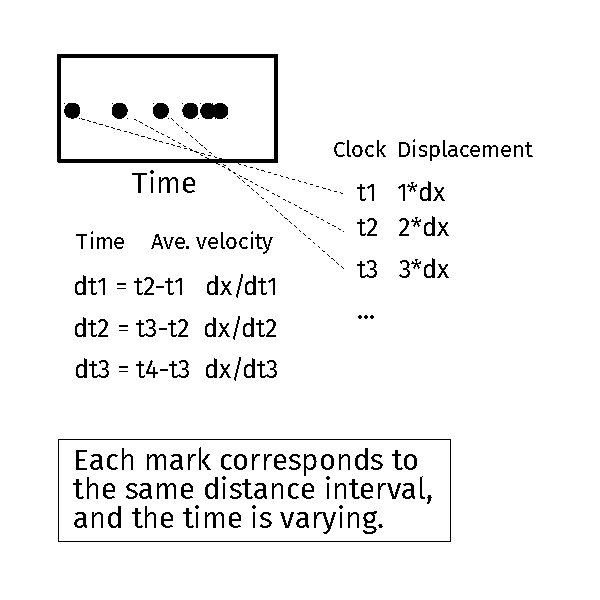
\includegraphics[width=0.55\textwidth]{figures/PicketG2.pdf}
\caption{\label{fig:picket2} We can measure the velocity versus time of the picket by taking the ratio of \textit{displacements} to \textit{times}.}
\end{figure}
\end{frame}

\begin{frame}{Lab Activity: Measuring acceleration of gravity}
\small
Acceleration is the change in velocity, so once we have the velocities ($dx/dt_{\rm i}$), we can take more ratios:
\begin{columns}[T]
\begin{column}{0.5\textwidth}
\begin{align}
t1' = (t2+t1)/2 & \quad dx/dt1 \\
t2' = (t3+t2)/2 & \quad dx/dt2 \\
t3' = (t4+t3)/2  & \quad dx/dt3 \\
...
\end{align}
\end{column}
\begin{column}{0.5\textwidth}
\begin{align}
t1' & \quad \frac{dx/dt2-dx/dt1}{t2'-t1'} \\
t2' & \quad \frac{dx/dt3-dx/dt2}{t3'-t2'}  \\
t3' & \quad \frac{dx/dt4-dx/dt3}{t4'-t3'}  \\
...
\end{align}
\end{column}
\end{columns}
\end{frame}

\begin{frame}{Lab Activity: Measuring acceleration of gravity}
Once we have the acclerations $\frac{dx/dt2-dx/dt1}{t2'-t1'}, ...$, we can compare them with each other and compute the \textit{average} and \textit{standard deviation}.\\
\begin{align}
\bar{a}_{\rm meas} &= N^{-1} \sum_{\rm i}^N a_{\rm meas,i} \\
\sigma^2_{\rm meas} &= N^{-1} \sum_{\rm i}^N (a_{\rm meas,i}-\bar{a}_{\rm meas})^2
\end{align} \\
Quote the result like this: $\bar{a}_{\rm meas}\pm\sigma_{\rm meas}$.  \textit{The mean plus or minus one standard deviation.}  The result of this experiment is $g = \bar{a}_{\rm meas}$, the acceleration due to gravity near the Earth's surface.
\end{frame}

\begin{frame}{Lab Activity: Measuring acceleration of gravity}
\small
\begin{figure}
\centering
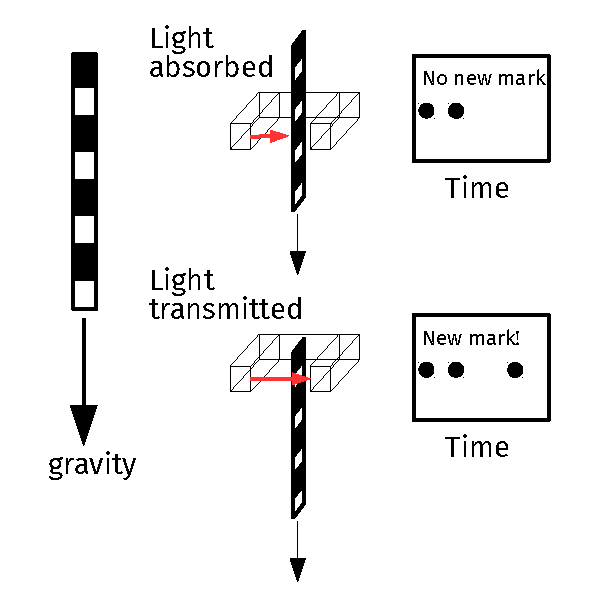
\includegraphics[width=0.5\textwidth]{figures/PicketG.pdf}
\caption{\label{fig:picket3} Does adding more mass to the picket change the answers?}
\end{figure}
\end{frame}

\section{Exercises with vectors, graphs, and equations of motion}

\begin{frame}{Exercises with vectors, graphs, and equations of motion}
We have a system of equations describing motion of classical particles undergoing constant acceleration:
\begin{align}
x &= x_{\rm 0} +\bar{v}t \\
\bar{v} &= (v+v_{\rm 0})/2 \\
v &= v_{\rm 0} + at \\
x &= x_{\rm 0} + v_{\rm 0} t + 	\frac{1}{2}at^2 \\
v^2 &= v_{\rm 0}^2 + 2a(x-x_{\rm 0})
\end{align}
\end{frame}

\begin{frame}{Exercises with vectors, graphs, and equations of motion}
A particle moves in a straight line with an initial velocity of 30 m/s and a constant acceleration of 30 m/s$^2$.  What is the displacement at $t=5$ seconds?  What is the velocity at $t=5$ seconds? \\
\begin{itemize}
\item A: 900 m, 180 m
\item B: 180 m, 525 m/s
\item C: 525 m, 180 m/s
\item D: 700 m, 200 m/s
\end{itemize}
\end{frame}

\begin{frame}{Exercises with vectors, graphs, and equations of motion}
A particle is moving at 5 m/s, 60 degrees with respect to the x-axis.  At $t=0$ seconds, it begins to accelerate at 1 m/s$^2$.  What is the speed after 3 seconds?\\
\begin{itemize}
\item A: 8 m/s
\item B: 4 m/s
\item C: -4 m/s
\item D: -8 m/s 
\end{itemize}
\end{frame}

\begin{frame}{Exercises with vectors, graphs, and equations of motion}
If the particle is at (0,0) at $t=0$, where is the particle at $t=3$ seconds? \\
\begin{itemize}
\item A: (7.5,13) m
\item B: (16.9,9.75) m
\item C: (9.75,16.9) m
\item D: (13,7.5) m 
\end{itemize}
\end{frame}

\begin{frame}{Exercises with vectors, graphs, and equations of motion}
\begin{columns}[T]
\begin{column}{0.4\textwidth}
\small
Which segment(s) of the motion described by the plot at right has $v\approx0$ (m/s)?
\begin{itemize}
\item A
\item B and D
\item C
\item E
\end{itemize}
\end{column}
\begin{column}{0.6\textwidth}
\begin{figure}
\centering
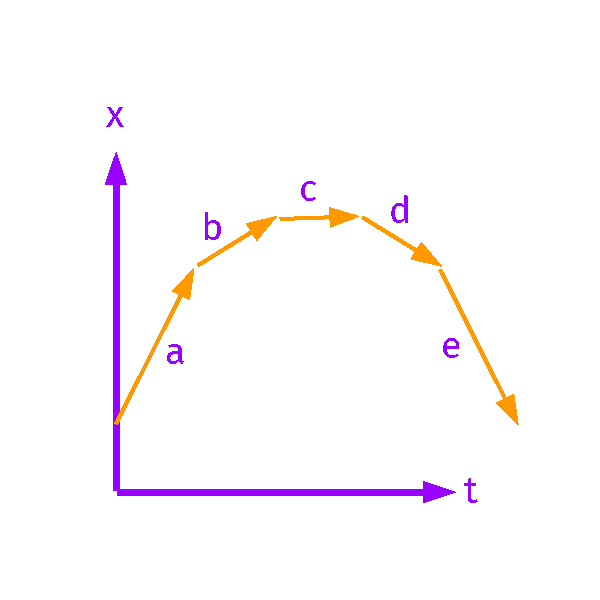
\includegraphics[width=\textwidth,trim=0cm 0cm 0cm 1.5cm,clip=true]{figures/Vectors2.pdf}
\end{figure}
\end{column}
\end{columns}
\end{frame}

\begin{frame}{Exercises with vectors, graphs, and equations of motion}
\begin{columns}[T]
\begin{column}{0.4\textwidth}
\small
Which segment(s) of the motion described by the plot at right has the largest velocity?
\begin{itemize}
\item A
\item B
\item D
\item E
\end{itemize}
\end{column}
\begin{column}{0.6\textwidth}
\begin{figure}
\centering
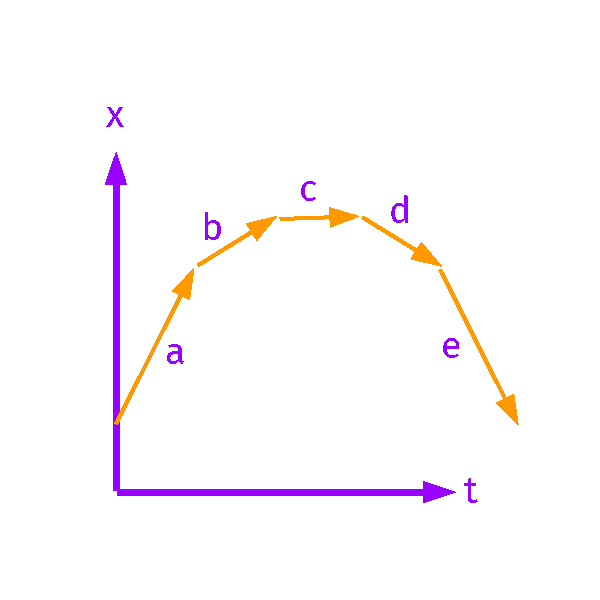
\includegraphics[width=\textwidth,trim=0cm 0cm 0cm 1.5cm,clip=true]{figures/Vectors2.pdf}
\end{figure}
\end{column}
\end{columns}
\end{frame}

\begin{frame}{Exercises with vectors, graphs, and equations of motion}
\begin{columns}[T]
\begin{column}{0.4\textwidth}
\small
Does the motion described by the plot correspond to negative or positive acceleration?
\begin{itemize}
\item Negative
\item Positive
\end{itemize}
\end{column}
\begin{column}{0.6\textwidth}
\begin{figure}
\centering
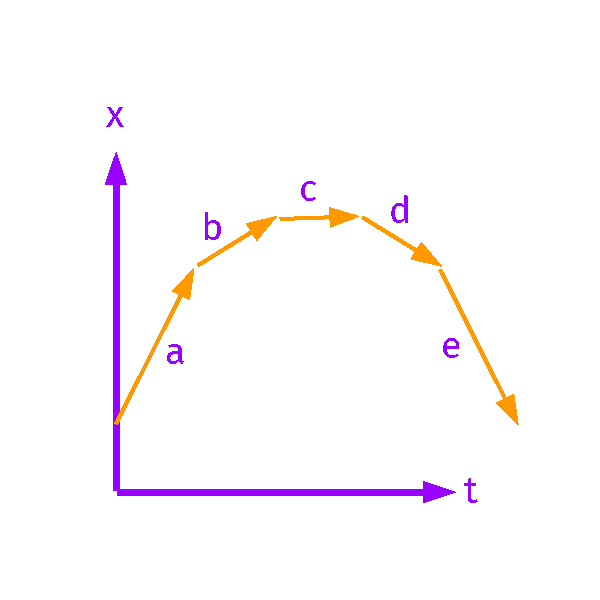
\includegraphics[width=\textwidth,trim=0cm 0cm 0cm 1.5cm,clip=true]{figures/Vectors2.pdf}
\end{figure}
\end{column}
\end{columns}
\end{frame}

\begin{frame}{Exercises with vectors, graphs, and equations of motion}
\begin{columns}[T]
\begin{column}{0.4\textwidth}
\small
In which region(s) is the acceleration zero m/s$^2$?
\begin{itemize}
\item A only
\item B only
\item Both A and B
\item None
\end{itemize}
\end{column}
\begin{column}{0.6\textwidth}
\begin{figure}
\centering
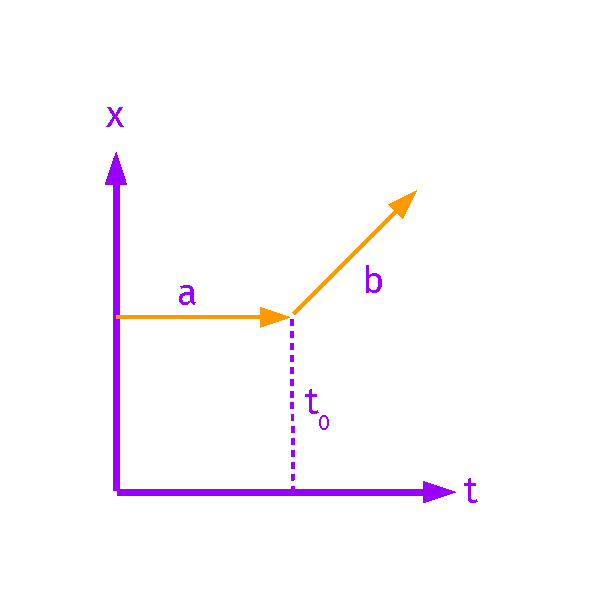
\includegraphics[width=\textwidth,trim=0cm 0cm 0cm 1.5cm,clip=true]{figures/Vectors3.pdf}
\end{figure}
\end{column}
\end{columns}
\end{frame}

\begin{frame}{Exercises with vectors, graphs, and equations of motion}
\begin{columns}[T]
\begin{column}{0.4\textwidth}
\small
At $t=t_{\rm 0}$, what is the acceleration?
\begin{itemize}
\item Negative and large
\item Positive and large
\item Positive, but small
\item Negative, but small
\end{itemize}
\end{column}
\begin{column}{0.6\textwidth}
\begin{figure}
\centering
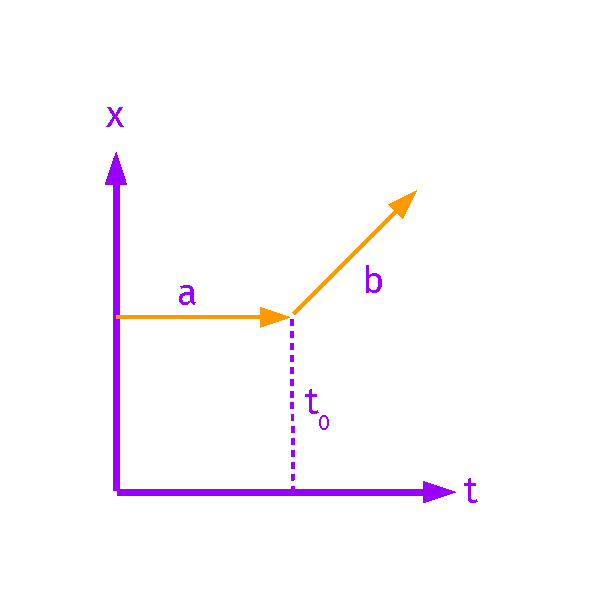
\includegraphics[width=\textwidth,trim=0cm 0cm 0cm 1.5cm,clip=true]{figures/Vectors3.pdf}
\end{figure}
\end{column}
\end{columns}
\end{frame}

\begin{frame}{Exercises with vectors, graphs, and equations of motion}
\begin{columns}[T]
\begin{column}{0.4\textwidth}
\small
What is the average velocity?
\begin{itemize}
\item Less than the slope of region B
\item Greater than the slope of region B
\item Zero
\end{itemize}
\end{column}
\begin{column}{0.6\textwidth}
\begin{figure}
\centering
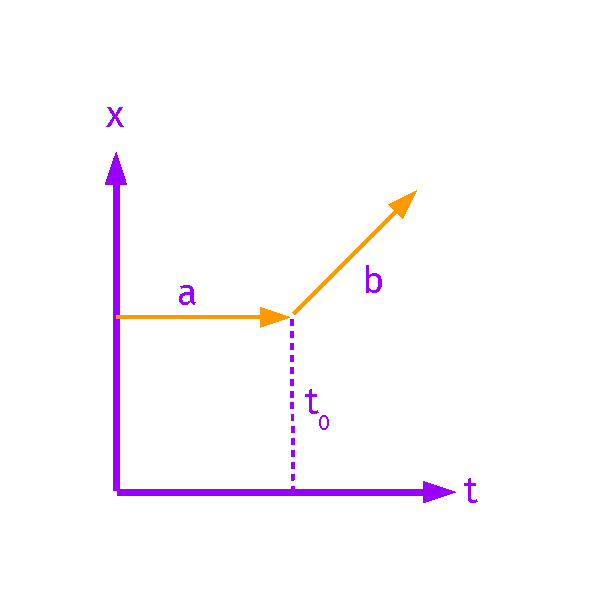
\includegraphics[width=\textwidth,trim=0cm 0cm 0cm 1.5cm,clip=true]{figures/Vectors3.pdf}
\end{figure}
\end{column}
\end{columns}
\end{frame}

\begin{frame}{Exercises with vectors, graphs, and equations of motion}
\begin{columns}[T]
\begin{column}{0.4\textwidth}
\small
What is the sign of the acceleration at $t=t_{\rm 1}$?  What is the sign of the acceleration at $t=t_{\rm 0}$?
\begin{itemize}
\item Negative, positive
\item Positive, negative
\item Positive, positive
\item Negative, negative
\end{itemize}
\end{column}
\begin{column}{0.6\textwidth}
\begin{figure}
\centering
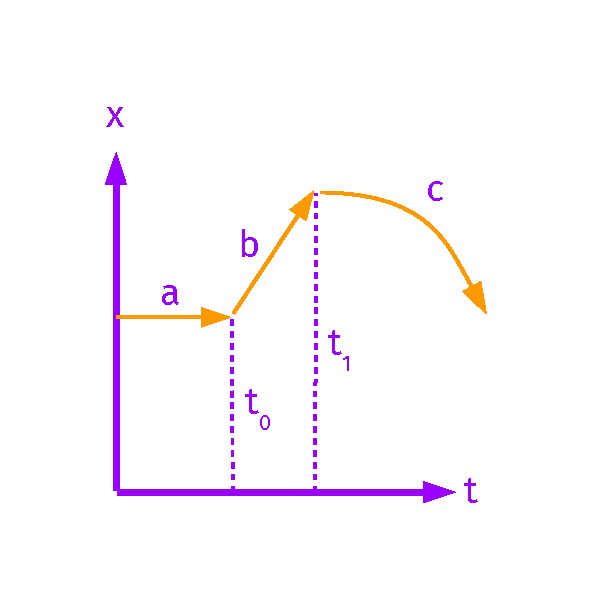
\includegraphics[width=\textwidth,trim=0cm 0cm 0cm 1.5cm,clip=true]{figures/FurtherExercises.pdf}
\end{figure}
\end{column}
\end{columns}
\end{frame}

\begin{frame}{Exercises with vectors, graphs, and equations of motion}
\begin{columns}[T]
\begin{column}{0.4\textwidth}
\small
What is most likely the total displacement?
\begin{itemize}
\item Positive and large
\item Negative and large
\item Zero
\item Cannot discern from graph
\end{itemize}
\end{column}
\begin{column}{0.6\textwidth}
\begin{figure}
\centering
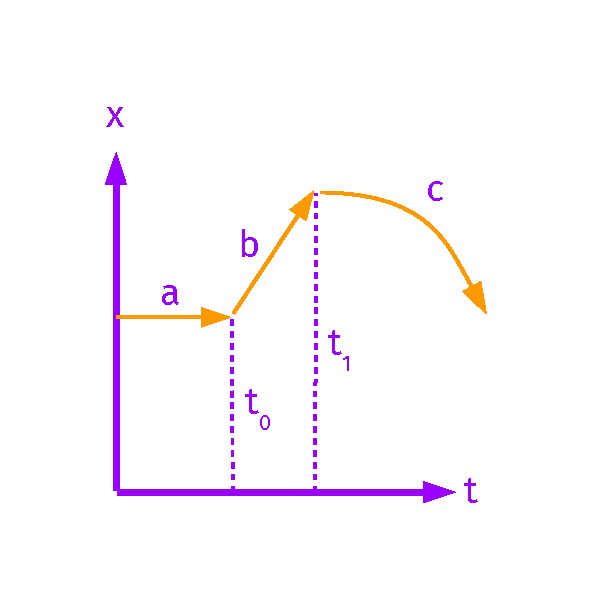
\includegraphics[width=\textwidth,trim=0cm 0cm 0cm 1.5cm,clip=true]{figures/FurtherExercises.pdf}
\end{figure}
\end{column}
\end{columns}
\end{frame}

\begin{frame}{Exercises with vectors, graphs, and equations of motion}
\begin{columns}[T]
\begin{column}{0.4\textwidth}
\small
What is most likely the acceleration during segment C?
\begin{itemize}
\item Positive and increasing
\item Negative and increasing
\item Negative and decreasing
\item Negative and constant
\end{itemize}
\end{column}
\begin{column}{0.6\textwidth}
\begin{figure}
\centering
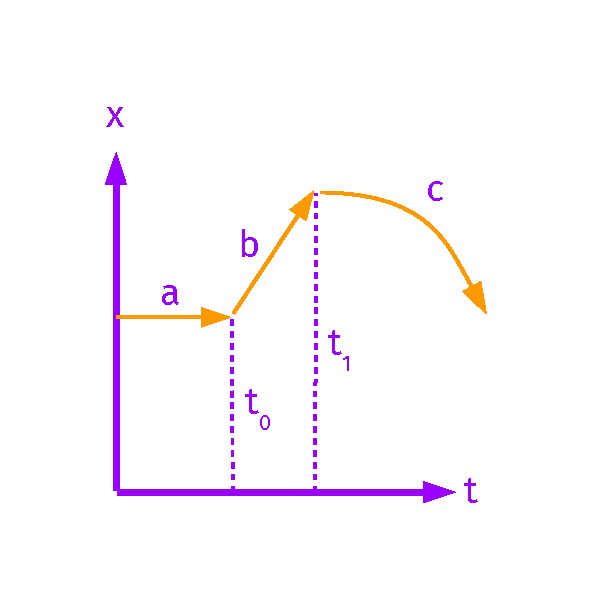
\includegraphics[width=\textwidth,trim=0cm 0cm 0cm 1.5cm,clip=true]{figures/FurtherExercises.pdf}
\end{figure}
\end{column}
\end{columns}
\end{frame}

\begin{frame}{Exercises with vectors, graphs, and equations of motion}
A particle is moving along the y-axis, with an initial speed of 10 m/s, and an acceleration of -10 m/s$^2$.  What is the displacement when the speed has decreased to 1 m/s?\\
\begin{itemize}
\item A: 3 m
\item B: 4 m
\item C: 5 m
\item D: 6 m
\end{itemize}
\end{frame}

\begin{frame}{Exercises with vectors, graphs, and equations of motion}
A particle is moving along the y-axis, with an initial speed of 10 m/s, and an acceleration of -10 m/s$^2$.  How much time has elapsed when the particle has a speed of 1 m/s?\\
\begin{itemize}
\item A: 0.9 seconds
\item B: 10 seconds
\item C: 0.5 seconds
\item D: 1.5 seconds
\end{itemize}
\end{frame}

\section{Conclusion}

\begin{frame}{Week 2 Summary}
\begin{enumerate}
\item Displacement, average velocity and acceleration
\begin{itemize}
\item \textit{Mathematics review}: slope of a function
\end{itemize}
\item The case of constant acceleration
\begin{itemize}
\item An \textit{an equation of motion} for constant acceleration
\item Derivation of \alert{common equations of motion}
\item Average quantities and exercises
\end{itemize}
\item \textbf{Lab Activity: Measuring acceleration of gravity: \textit{g}}
\item Exercises with vectors, graphs, and equations of motion
\end{enumerate}
\end{frame}

\end{document}
